%& -job-name=DDN_Lustre_version-matrix
\documentclass{article}
\usepackage[utf8]{inputenc}
\usepackage{setspace}
\usepackage{graphicx}
\usepackage{dirtree}
\usepackage[hang]{footmisc}
\usepackage{vhistory}
\renewcommand{\hangfootparskip}{10pt}
\setlength{\skip\footins}{1cm}
\setlength{\parskip}{1em}
\usepackage[a4paper, total={6in, 8in}]{geometry}


\title{%
Lustre File System - OS Compatibility Matrix \\
\large Zenuity Oden Cluster (NGSC)}
\author{Carlos Thomaz - cthomaz@ddn.com}
\date{\today}
\begin{document}

\maketitle


\begin{center}
    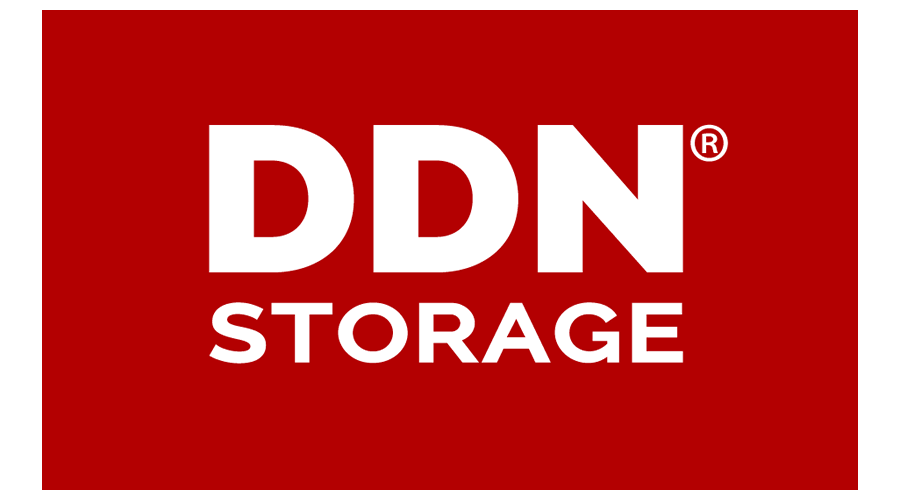
\includegraphics[scale=0.14]{logo.png}\\[1cm] 
\end{center}

\newpage

\begin{versionhistory}
    \vhEntry{Draft}{05.13.20}{CT}{Initial version}
    \vhEntry{v1.0}{05.14.20}{CT}{v1.0 - Current compat. matrix}
    \vhEntry{v1.1}{05.14.20}{CT}{v1.1 - DMF nodes version fixed}
    \vhEntry{v1.2}{05.18.20}{CT}{v1.2 - SLES 12 SP5 support request placeholder}
\end{versionhistory}


\newpage
\section{Introduction}
This document describes the Operating System compatibility matrix including dependencies and other details that ensures the supportability of Lustre file system. This matrix are subjected to change during the course of the project. 

\section{DDN Exascaler - Server Side}
The initial project rollout will be based on DDN Exascaler 5.1. The stack will be rolled out on \textbf{server side}  as it is, without any modifications\footnote{Lustre or other OS component patching}. Exascaler 5.1 is based on the following main software components. 
\begin{table}[h]
 \centering
 \begin{tabular}{||l l l||}
 \hline
 \textbf{Component} & \textbf{Description} & \textbf{Version} \\ [0.5ex] 
 \hline\hline
 Operating System & CentOS & 7.7 \\ 
 \hline
 OS Kernel & Linux & 3.10.0-1062 \\
 \hline
 RDMA support & Mellanox OFED & 4.7.3.2.9.1 \\
 \hline
 File System & Lustre & 2.12.3-ddn8 \\
 \hline
 HCA & Mellanox EDR HCA firmware & 16.26.1040 \\
 \hline
 DDN storage & SFAOS version & 11.7.0 \\
 \hline
 \end{tabular}
 \caption{DDN Exascaler - Lustre Server Side}
 \label{tab:os-compat-serverside}
\end{table}

If a need for patching Lustre is identified, a process will be taken in place to upgrade the necessary component assuring the DDN / Whamcloud engineering support.

\section{Lustre clients}
It's been decided that Lustre clients must be supported on two different OS distributions. One to be used by the compute client nodes, running SuSE Linux and Lustre clients running RedHat derived distributions (CentOS) where HPE DMF will be installed. There are different supported software stack for each one of the \textit{flavors} of clients.

\subsection{Compute Nodes - SuSE Linux based}
Generic compute nodes will run SuSE Enterprise Linux distribution. The following table defines the exact versions required to be provisioned on these nodes to guarantee full interoperability and support. 
\begin{table}[h]
 \centering
 \begin{tabular}{||l l l||}
 \hline
 \textbf{Component} & \textbf{Description} & \textbf{Version} \\ [0.5ex] 
 \hline\hline
 Operating System & SuSE Linux Enteprise Edition & 12 SP4\\ 
 \hline
 OS Kernel & Linux & 4.12.14-94.41.1 \\
 \hline
 RDMA support & Mellanox OFED & 4.7.3.2.9.1 \\
 \hline
 File System & Lustre & 2.12.3-ddn8 \\
 \hline
 HCA & Mellanox EDR HCA firmware & tbd \\
 \hline
 \end{tabular}
 \caption{DDN Exascaler - Lustre Client Side - Generic Compute Nodes}
 \label{tab:os-compat-clientside-generic}
\end{table}

\subsection{DMF Nodes - RedHat Enterprise Linux}
HPE DMF is considered Lustre client. These nodes will run CentOS due DMF interoperability requirements. For this class of clients the following versions should be considered in order to guarantee full interoperability and support.

\begin{table}[h]
 \centering
 \begin{tabular}{||l l l||}
 \hline
 \textbf{Component} & \textbf{Description} & \textbf{Version} \\ [0.5ex] 
 \hline\hline
 Operating System & RHEL & 7.7\\ 
 \hline
 OS Kernel & Linux & 3.10.0-1062 \\
 \hline
 RDMA support & Mellanox OFED & 4.7.3.2.9.1 \\
 \hline
 File System & Lustre & 2.12.3-ddn8 \\
 \hline
 HCA & Mellanox EDR HCA firmware & tbd \\
 \hline
 \end{tabular}
 \caption{DDN Exascaler - Lustre Client Side - DMF Nodes}
 \label{tab:os-compat-clientside-dmf}
\end{table}

\subsection{Infiniband HCA firwmare on compute nodes}
All compute nodes and external servers are provided by HPE and must run the supported Mellanox or Mellanox OEM firmware compatible with the Infiniband Stack defined in this document. 

\subsection{Lustre client support}
DDN will provide the source code for Lustre clients. It is imperative to run the versions supported and recommended by DDN in order to honor the compatibility matrix and continue being fully supported by DDN and Whamcloud engineering. The utilization of Lustre community releases (cloned or downladed from public GIT repositories) are not encouraged and will void support.

DDN will also provide patches and Lustre clients if needed. The \textbf{-ddn8} tag is the default version for Exascaler 5.1. However, as best practice, DDN may provide a different source code that may contain fixes and performance patches.

\section{Future requests}
HPE has requested support for SLES 12 SP5 due the possibility of SLES 12 SP4 going End-of-support soon. Whamcloud is tracking this request under DDN internal JIRA ticket \textbf{DDN-1261}. Whamcloud is proposing support for SLES 12 SP5 done with ES5.1.1 release, targeted to June time-frame. 

\end{document}
